\subsection{Sơ đồ ca sử dụng}
% https://www.uml-diagrams.org/use-case-diagrams.html

\begin{figure}[h!]
	\centering
	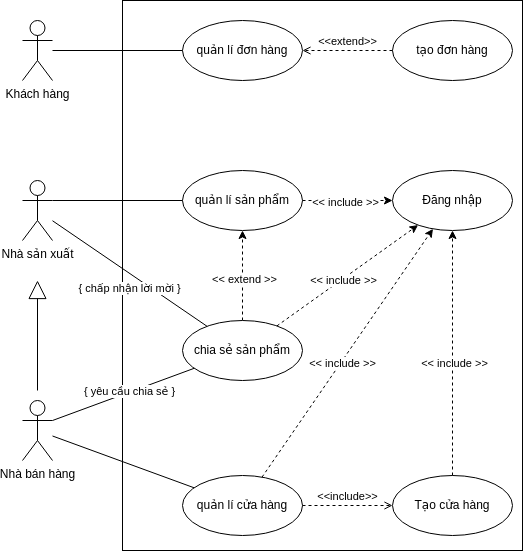
\includegraphics[width=0.6\textwidth]{usecase-usecase}
	\caption{Sơ đồ ca sử dụng tổng quát}
\end{figure}

\begin{figure}[h!]
	\begin{center}	
		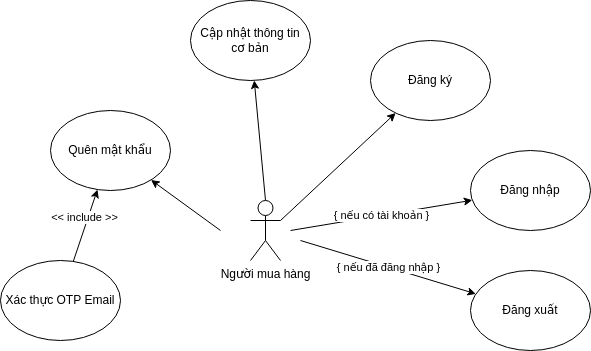
\includegraphics[width=0.6\textwidth]{usecase-user-login}
		\caption{Sơ đồ ca đăng nhập}
	\end{center}
\end{figure}


\begin{figure}[h!]
	\begin{center}	
		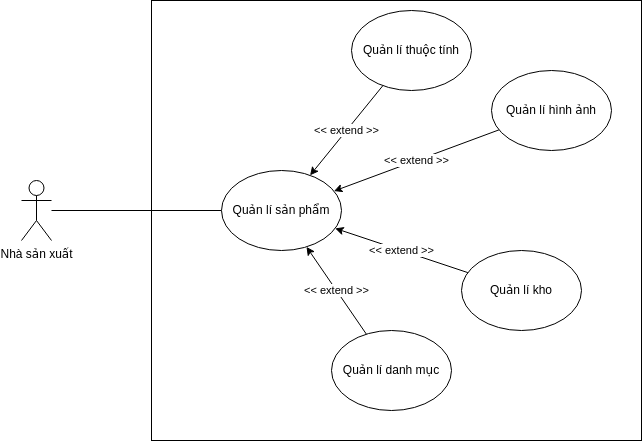
\includegraphics[width=0.6\textwidth]{usecase-sellers}
		\caption{Sơ đồ ca quản lí sản phẩm}
	\end{center}
\end{figure}


\begin{figure}[h!]
	\begin{center}	
		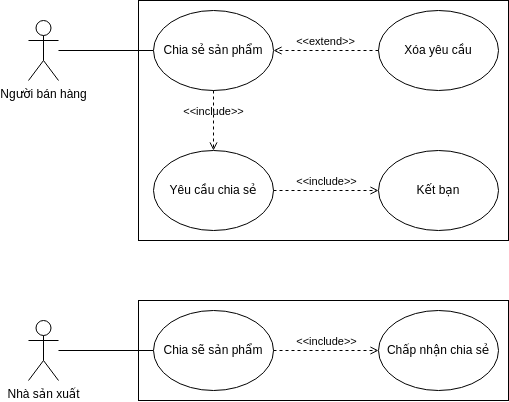
\includegraphics[width=0.6\textwidth]{usecase-contract}
		\caption{Sơ đồ ca yêu cầu chia sẻ}
	\end{center}
\end{figure}


\begin{figure}[h!]
	\begin{center}	
		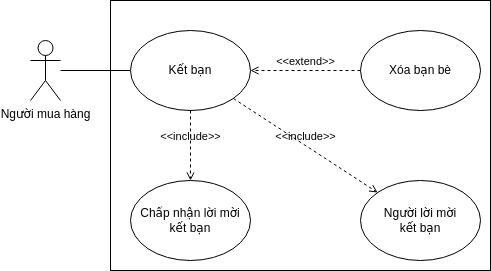
\includegraphics[width=0.6\textwidth]{usecase-relationship}
		\caption{Sơ đồ ca trường hợp kết bạn}
	\end{center}
\end{figure}



\begin{figure}[h!]
	\begin{center}	
		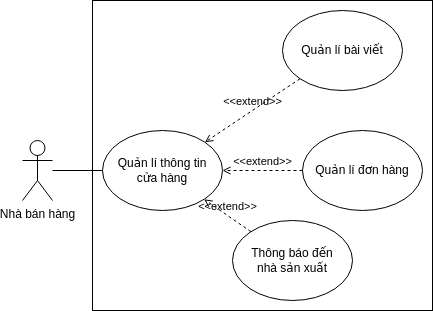
\includegraphics[width=0.5\textwidth]{usecase-store}
		\caption{Sơ đồ ca trường hợp quản lí cửa hàng}
	\end{center}
\end{figure}

\begin{figure}[h!]
	\begin{center}	
		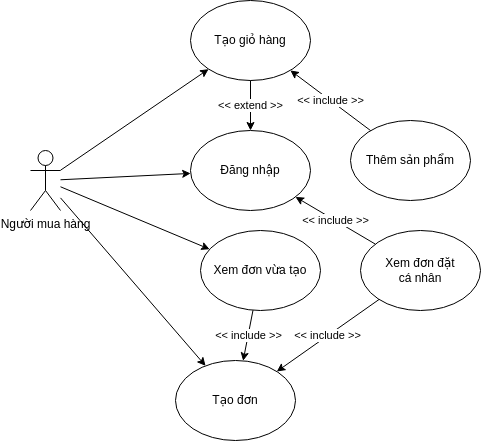
\includegraphics[width=0.6\textwidth]{usecase-order}
		\caption{Sơ đồ ca đặt hàng}
	\end{center}
\end{figure}

% Tính năng chia sẻ là khi lời mời được chấp nhận, sản phẩm của trang thương mại điện tử này có thể hiển thị và đặt mua ở trên trang khác. Nếu có cập nhật thì sản phẩm sẽ tự động đồng bộ.

\begin{figure}[h!]
	\begin{center}	
		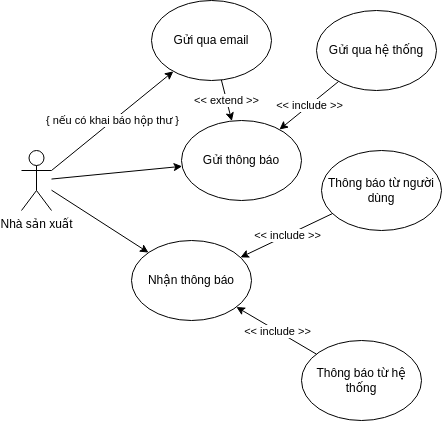
\includegraphics[width=0.5\textwidth]{usecase-notification}
		\caption{Sơ đồ ca trường hợp thông báo}
	\end{center}
\end{figure}